\section{Evaluation}
\label{sec:Evaluation}

\subsection{Datasets}

We evaluate our method on two complementary benchmarks that together cover synthetic, large-scale variation and high-fidelity real scans.  First, Anomaly-ShapeNet is a synthetic point-cloud benchmark built on top of ShapeNetCoreV2 and intended to provide diverse, controllable defect examples for 3D anomaly detection \cite{li2024towards,chang2015shapenet}.  The released benchmark used in this paper contains 1,600 samples across 40 object categories. The authors synthesize six realistic defect types, namely bulge, concavity, hole, break, bending, and crack, with the anomalous region occupying about one to ten percent of the points in affected samples.  Defects are created using Blender sculpting tools and the corresponding point-level ground truth masks are generated by geometric comparison tools and exported with CloudCompare \cite{li2024towards}.

Second, Real3D-AD is a high-precision, real-scan dataset collected for industrial 3D anomaly detection and benchmarking \cite{liu2023real3d}. Real3D-AD contains 1,254 scanned objects spanning 12 categories (for example, airplane, car, candybar, diamond, seahorse and toffees).  The point clouds are high density, with per-object point counts ranging from tens of thousands to on the order of two million points, and a point-to-point sampling resolution on the order of 0.0010 mm to 0.0015 mm.  Scans were captured using a blue-light structured-light scanner (PMAX-S130) on a rotating turntable to obtain full 360 degree coverage; defects were labeled using a CloudCompare-based pipeline that leverages octree comparison plus manual verification to produce per-point anomaly masks \cite{liu2023real3d}.  The dataset is organized in a prototype-based training setup: each class provides a small set of pristine prototypes for training and separate test folders containing both normal and defective scans together with ground-truth masks and text annotations, which makes Real3D-AD suitable for evaluating prototype-driven and registration-based anomaly methods.

\subsection{Implementation Details}
\label{sec:impl}

We implement the complete framework in PyTorch\footnote{Code and dataset: \url{https://github.com/hoangcuongbk80/Mamba3dAD}} and execute all experiments on a workstation equipped with four NVIDIA RTX 3090 GPUs (24\,GB each). Training is performed with mixed precision using NVIDIA AMP and with PyTorch Distributed Data Parallel (DDP) across the four devices. To improve reproducibility we fix the global random seed to 42 and control nondeterministic sources where possible; by default we keep cuDNN’s nondeterministic kernels enabled for throughput, but experiments that require bitwise reproducibility can force deterministic behavior. Checkpoints, training logs, and evaluation scripts are provided in the public repository.

All raw scans are preprocessed with voxel-grid filtering to keep memory and compute tractable: we use a voxel size of 0.0005\,m for Real3D-AD and 0.001\,m for Anomaly-ShapeNet, matching the dataset recommendations. After voxelization each cloud is translated to zero mean and scaled to unit radius. During training we apply on-the-fly augmentations before patch extraction: random yaw rotation sampled uniformly in $[0,2\pi)$, isotropic Gaussian jitter with standard deviation $\sigma=0.005$\,m (clipped at $2\sigma$), uniform scaling in the range $[0.95,1.05]$, light point dropout up to 5\% of points, and a small random translation $\pm 0.002$\,m. These augmentations increase robustness while preserving patch identity across Transformer layers within a forward pass.

Patch extraction uses Farthest Point Sampling (FPS) to select $M=256$ patch centers and $K$-nearest neighbors with $K=512$ points per patch, unless noted otherwise. Each neighborhood is encoded by a lightweight PointNet-style encoder followed by a two-layer positional-encoding MLP to produce patch embeddings of dimension $D$, where $D$ is set to match the pretrained Transformer token size (Point-MAE defaults to $D=768$ in our experiments). The Transformer backbone (Point-MAE pretrained on ShapeNet) is kept frozen in all runs; only the Geometric Semantic-Aware Sorter (GSAS), the Mamba adapter, the positional-MLP, the anomaly-scaling scalar $\gamma$, and the attention discriminator are trainable. For extremely large scans (e.g., Real3D objects that produce very high $T$ after unfolding layers and patches) we reduce $M$ or increase the voxel size during preprocessing to keep memory usage bounded.

The GSAS intra-layer aggregation descriptor dimension is $d_a=128$. Token-slot logits are produced by a linear layer $W_{\uparrow}\in\mathbb{R}^{d_a\times T}$ where $T=L\cdot M$ is the total token count across all backbone layers; in practice $T$ ranges from a few thousand up to tens of thousands depending on the backbone depth $L$ and patch count $M$. For the Sinkhorn soft-permutation we use temperature $\tau=0.05$ and $K_{\mathrm{sink}}=20$ iterations; the geometric-affinity bandwidth is set to $\sigma_p=0.05$ in unit-radius coordinates, and numerical stability values are $\epsilon_{\mathrm{ent}}=\epsilon_{\mathrm{norm}}=10^{-8}$. Reasonable default weights for the auxiliary regularizers are $\alpha_{\mathrm{ent}}=10^{-2}$ and $\alpha_{\mathrm{loc}}=10^{-1}$; these coefficients are tuned on the validation split. When a crisper ordering is desired for deployment we lower $\tau$ and/or increase $K_{\mathrm{sink}}$, and for very long sequences the Sinkhorn iterations can be truncated or replaced by blockwise assignment to trade off runtime and ordering accuracy.

The Mamba adapter uses a latent state size $S=256$ in our default configuration. To promote stable recurrent dynamics we initialize $A$ as a scaled identity with spectral radius close to one (we use $A\approx 0.98\,I_S$ with small Gaussian perturbations) and initialize $B,C,D$ with Kaiming normal initialization and small biases. These simple initialization choices proved reliable across datasets; substituting HiPPO-inspired parameterizations is also supported if desired. With the chosen $S$ and $D$, the adapter contributes a modest parameter overhead, typically under 5\% relative to the frozen backbone.

During training the anomalous feature generator corrupts tokens sparsely to emulate localized defects. We set the corruption probability to $p=0.05$ by default and sample isotropic Gaussian perturbations with scale $\sigma=0.1$; the adaptive rescaling parameter $\gamma$ is learned but initialized to $0.1$. To mitigate class imbalance induced by sparse corruption we either set the BCE-with-logits positive-class weight \texttt{pos\_weight} to $(1-p)/p$ or tune a scalar $w_{+}$ on the validation split. The primary training objective is the numerically-stable logits-based binary cross-entropy averaged across supervised slots, augmented by the entropy and locality regularizers from GSAS.

The attention-based discriminator uses $H=8$ heads and a two-layer MLP head with hidden size $D/2$ and GELU activation. Dropout with rate 0.1 and layer normalization are applied inside the attention block and MLP head to stabilize optimization. If $D$ is not divisible by $H$ we apply a thin linear projection to the nearest divisible dimension to avoid per-head mismatches. All trainable modules are optimized jointly with AdamW using initial learning rate $1\times 10^{-4}$, weight decay $1\times 10^{-2}$, and $\beta=(0.9,0.999)$. We perform a 2-epoch linear warmup from $1\times 10^{-5}$ followed by cosine annealing to zero over 100 epochs. Batch size is 8 total across GPUs in our standard runs (two samples per GPU); we clip gradients to norm 1.0 and use 8 dataloader workers per GPU to balance IO and CPU preprocessing.

At inference time the anomalous feature generator is disabled and the pipeline is deterministic: extract voxelized patches and centers, compute frozen-transformer tokens, apply GSAS to obtain an ordering, run the Mamba adapter to produce adapted tokens, add coordinate-derived positional embeddings, and evaluate the attention discriminator to obtain per-slot logits. We map per-slot logits back to points by taking the maximum score among the patches that contain each point and optionally apply a 3D median filter in voxel space for spatial smoothing; voxel-filter parameters and detection/segmentation thresholds ($\tau_{\mathrm{pc}}$, $\tau_{\mathrm{seg}}$) are selected on validation. For deployments that require deterministic hard orderings we optionally discretize the soft permutation using the Hungarian algorithm on $-\mathbf{G}$; for latency-sensitive settings one may instead reduce $K_{\mathrm{sink}}$, run GSAS blockwise, or cache the patch-extraction step for static objects.

%-------------------------------------------------------
\begin{figure}[!ht]
    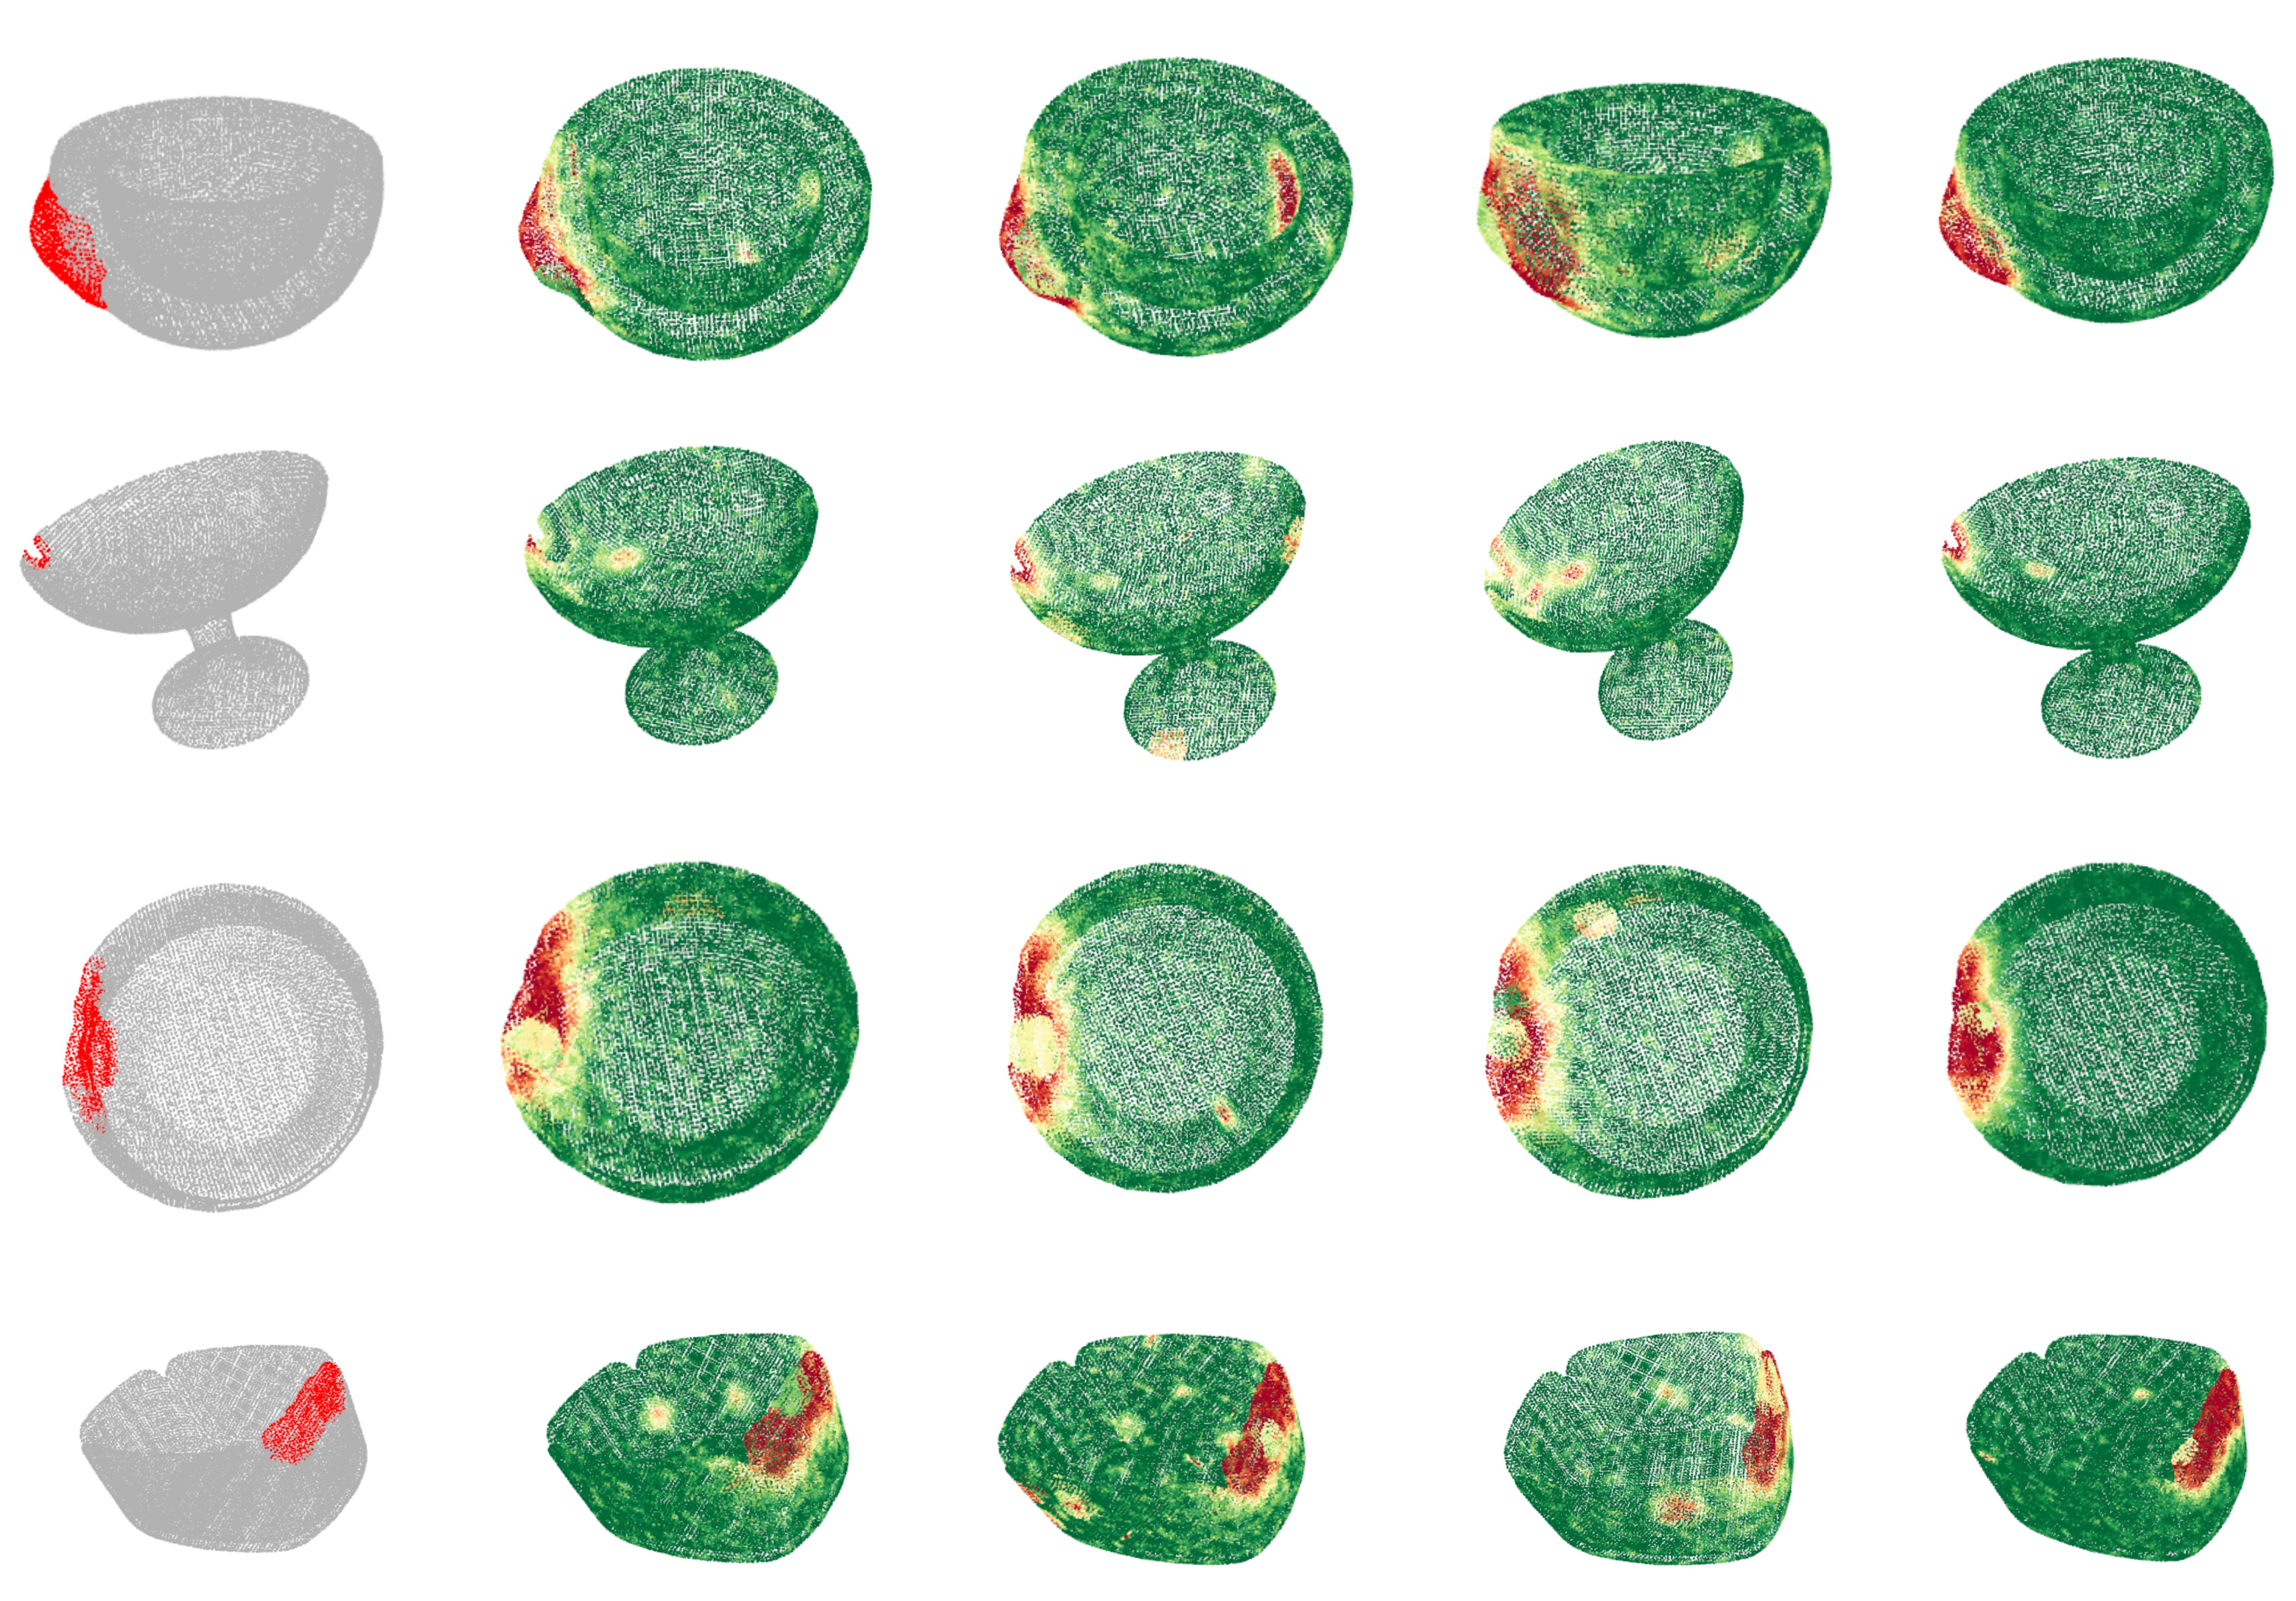
\includegraphics[width=\linewidth]{figs/shapenet}  
    Input + GT \hspace{1.2cm} 3D-ST \cite{bergmann2023anomaly} \hspace{1.3cm} Reg3D-AD \cite{liu2023real3d} \hspace{1.5cm} Group3AD   \cite{zhu2024towards} \hspace{1.7cm} Ours \hspace{0.8cm}
    \caption{Qualitative results on the newly collected Anomaly-ShapeNet \cite{li2024towards}. From left to right: input point clouds and ground truth annotations of anomalous points in red, and anomaly scores for each 3D point predicted by the proposed method.}
    \label{fig:shapenet}
\end{figure}
%-------------------------------------------------------
  
%-------------------------------------------------------
\begin{figure}[!ht]
    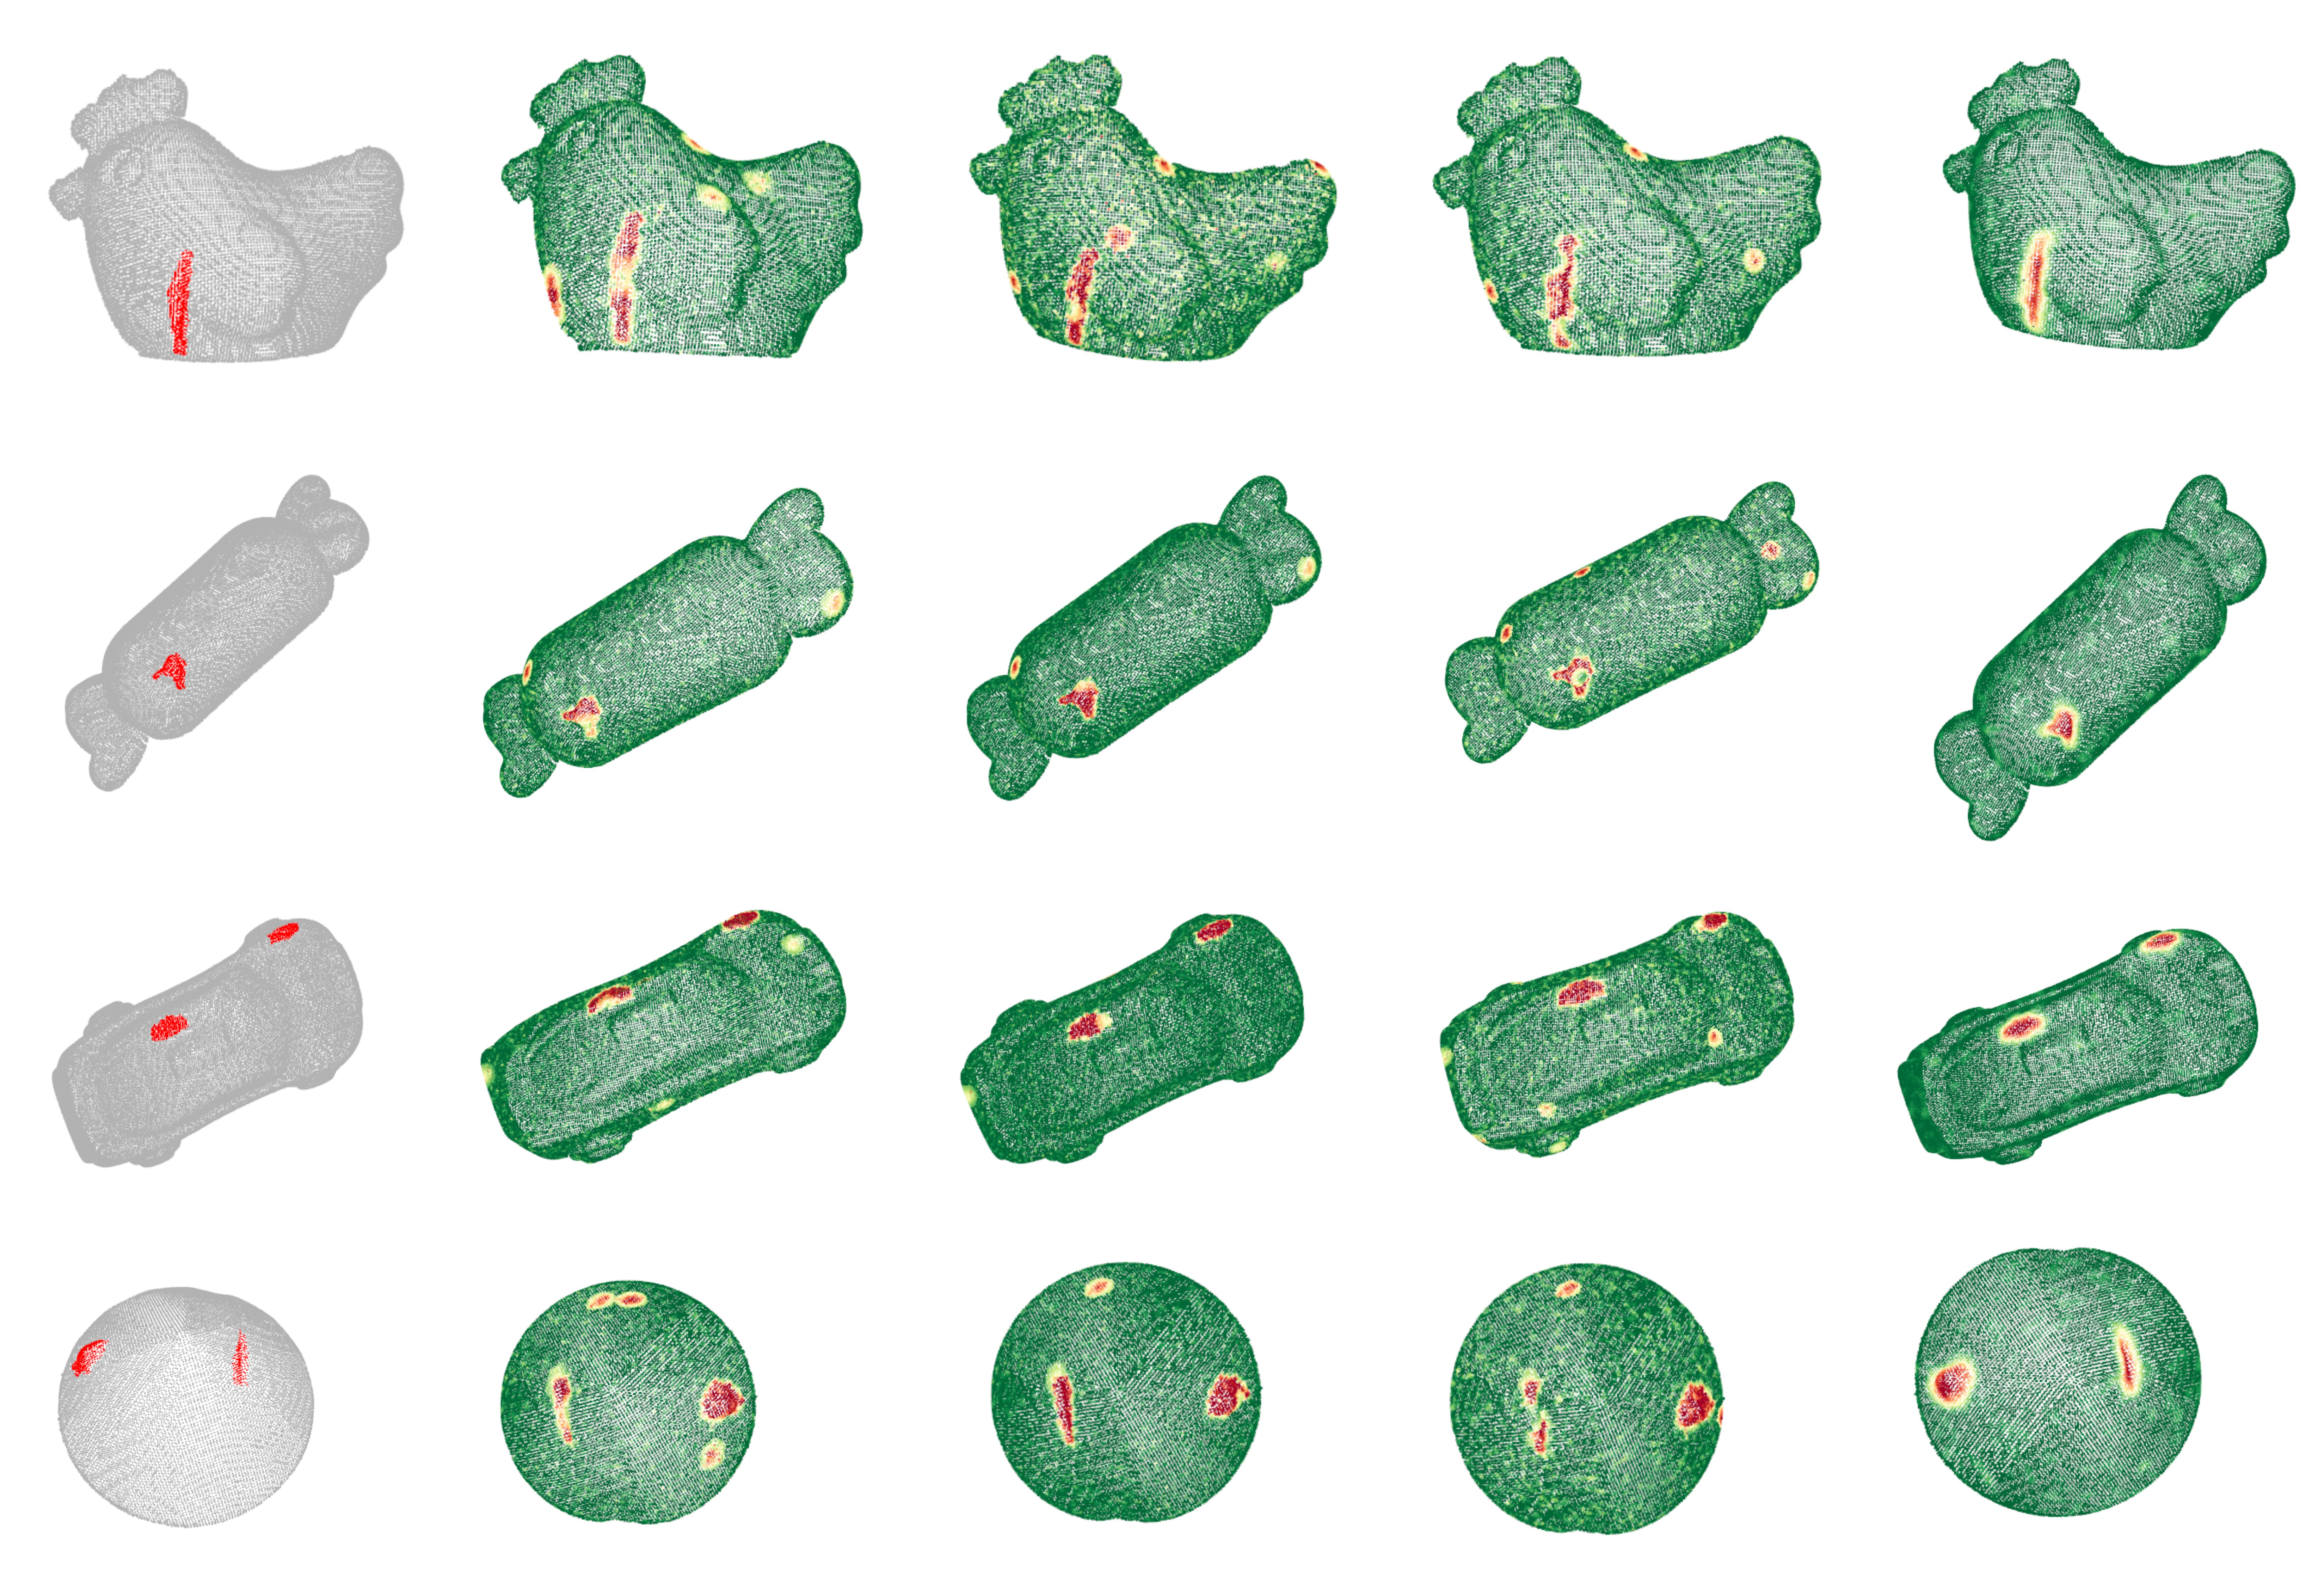
\includegraphics[width=\linewidth]{figs/real3d}
    Input + GT \hspace{1.2cm} 3D-ST \cite{bergmann2023anomaly} \hspace{1.3cm} Reg3D-AD \cite{liu2023real3d} \hspace{1.3cm} Group3AD   \cite{zhu2024towards} \hspace{1.7cm} Ours \hspace{1.5cm}
    \caption{Qualitative results on Real3D-AD dataset. From left to right: input point clouds, Ground truth annotations of anomalous points in red, and anomaly scores for each 3D point predicted by the proposed method.}
    \label{fig:real3d}
\end{figure}
%-------------------------------------------------------

\subsection{Evaluation Metrics}

We assess the performance of anomaly detection models using both object-level and point-level evaluation metrics derived from the receiver operating characteristic (ROC) and precision–recall (PR) curves. These complementary measures capture different aspects of detection performance: ROC-based metrics emphasize overall discrimination capability, while PR-based metrics are more sensitive to rare positive instances, as is typical in anomaly detection.

The ROC curve characterizes the trade-off between sensitivity and specificity by plotting the true positive rate (TPR) against the false positive rate (FPR) as the decision threshold varies. Let $\mathrm{TP}$, $\mathrm{FP}$, $\mathrm{TN}$, and $\mathrm{FN}$ denote the number of true positives, false positives, true negatives, and false negatives, respectively. The TPR and FPR are defined as
\begin{equation}
\mathrm{TPR} = \frac{\mathrm{TP}}{\mathrm{TP} + \mathrm{FN}}, 
\qquad
\mathrm{FPR} = \frac{\mathrm{FP}}{\mathrm{FP} + \mathrm{TN}}.
\end{equation}
The area under the ROC curve (AUROC) summarizes the ROC curve into a single scalar measure,
\begin{equation}
\mathrm{AUROC} = \int_{0}^{1} \mathrm{TPR}(\mathrm{FPR})\,\mathrm{d}\mathrm{FPR},
\end{equation}
where an AUROC of 0.5 indicates random guessing, and a score of 1.0 denotes perfect discrimination. AUROC is threshold-independent and robust to class imbalance, which makes it widely used for both binary classification and anomaly detection.

While AUROC evaluates general separability between normal and anomalous samples, the PR curve focuses on the model’s effectiveness in identifying the positive (anomalous) class. Precision and recall are defined as
\begin{equation}
\mathrm{Precision}\ (P) = \frac{\mathrm{TP}}{\mathrm{TP} + \mathrm{FP}}, 
\qquad
\mathrm{Recall}\ (R) = \frac{\mathrm{TP}}{\mathrm{TP} + \mathrm{FN}}.
\end{equation}
The area under the precision–recall curve (AUPR) is computed as
\begin{equation}
\mathrm{AUPR} = \int_{0}^{1} P(R)\,\mathrm{d}R,
\end{equation}
providing a threshold-independent measure of anomaly retrieval performance. Because the baseline precision corresponds to the fraction of anomalies in the dataset, AUPR is particularly informative in highly imbalanced scenarios, reflecting a model’s ability to retrieve true anomalies while minimizing false detections.

At the \textbf{object level}, each point cloud is treated as a single instance. A global anomaly score is typically obtained by aggregating per-point anomaly scores, for example using the maximum response across all points in the cloud. Object-level AUROC and AUPR are then computed over the entire set of test point clouds. At the \textbf{point level}, each point’s predicted score is directly compared with its binary ground-truth label, yielding fine-grained evaluation of spatial localization performance. Together, these metrics provide a comprehensive assessment of both detection accuracy and localization precision across scales.

\subsection{Result}

%-------------------------------------------------------

\begin{table}[ht]
\centering
\caption{Average Result (\%) on Anomaly-ShapeNet dataset.}
\label{tab:ShapeNet}
\begin{tabular}{l|cc|cc|c}
\hline
& \multicolumn{2}{c|}{Point Level (\%)} & \multicolumn{2}{c|}{Object Level (\%)} & Speed \\
\hline
& AUROC & AUPR & AUROC & AUPR & FPS \\ 
\hline
BTF(Raw)                            & 55.2 & 16.4  & 49.5 & 57.4  & 2.09 \\ 
BTF(FPFH)                           & 63.0 & 21.0  & 53.1 & 61.0  & 1.16 \\ 
M3DM(PointMAE)                      & 61.8 & 21.5  & 55.4 & 61.4  & 0.31 \\ 
M3DM(PointBERT)                     & 60.3 & 19.5  & 53.7 & 59.6  & 0.52 \\ 
PatchCore(FPFH)                     & 58.2 & 21.1  & 57.1 & 61.0  & 0.10 \\ 
PatchCore(FPFH+Raw)                 & 60.4 & 22.3  & 58.6 & 63.2  & 0.10 \\ 
PatchCore(PointMAE)                 & 57.9 & 19.4  & 56.4 & 59.3  & 0.12 \\ 
Reg3D-AD \cite{liu2023real3d}       & 67.0 & 20.3  & 57.4 & 70.3  & 0.10 \\ 
3D-ST \cite{bergmann2023anomaly}    & 63.6 & 22.6  & 60.7 & 60.5  & 1.52 \\
Group3AD \cite{zhu2024towards}      & 84.6 & 25.4  & 81.4 & 95.3  & 2.55 \\ 
IMRNet \cite{li2024towards}         & 65.3 & 22.8  & 66.3 & 72.7  & 5.62 \\
R3D-AD \cite{zhou2024r3d}           & 75.1 & 23.7  & 75.2 & 73.6  & 7.15 \\
Ours                                & 91.2 & 38.7  & 86.8 & 98.7  & 17.31 \\
\hline
\end{tabular}
\end{table}

%-------------------------------------------------------

%-------------------------------------------------------

\begin{table}[ht]
\centering
\caption{Average Results (\%) on Real3D-AD dataset.}
\label{tab:Real3D}
\begin{tabular}{l|cc|cc|c}
\hline
& \multicolumn{2}{c|}{Point Level (\%)} & \multicolumn{2}{c|}{Object Level (\%)} & Speed \\
\hline
& AUROC & AUPR & AUROC & AUPR & FPS \\ 
\hline
BTF(Raw)                            & 57.3 & 2.4 & 60.5 & 61.3  & 2.05 \\
BTF(FPFH)                           & 73.2 & 6.6 & 63.7 & 61.6  & 1.01 \\
M3DM(PointMAE)                      & 63.9 & 4.9 & 55.4 & 57.5  & 0.31 \\
M3DM(PointBERT)                     & 63.9 & 5.4 & 54.0 & 58.3  & 0.52 \\
PatchCore(FPFH)                     & 57.9 & 7.3 & 59.6 & 59.3  & 0.10 \\
PatchCore(FPFH+Raw)                 & 68.2 & 12.5 & 68.4 & 66.9  & 0.10 \\
PatchCore(PointMAE)                 & 64.5 & 6.0 & 59.6 & 63.6  & 0.12 \\
Reg3D-AD \cite{liu2023real3d}       & 70.7 & 11.1 & 70.7 & 72.6  & 0.10 \\
3D-ST \cite{bergmann2023anomaly}    & 70.7 & 11.1 & 64.8 & 72.6  & 1.52 \\
Group3AD   \cite{zhu2024towards}    & 73.8 & 13.9 & 75.3 & 74.3  & 2.55 \\
IMRNet   \cite{li2024towards}       & 72.8 & 16.8 & 72.8 & 62.8  & 5.62 \\
R3D-AD   \cite{zhou2024r3d}         & 59.4 & 4.3 & 73.6 & 63.5  & 7.15 \\
Ours                                & 76.6 & 19.7 & 78.4 & 77.7 & 17.31 \\
\hline
\end{tabular}
\end{table}

%-------------------------------------------------------


Figures \ref{fig:result1} and \ref{fig:result2} present qualitative segmentation results on the Real3D-AD and Industrial3D-AD benchmarks, respectively, illustrating the model's ability to localize both bulges and sinks in high-precision scans and to robustly highlight subtle scratches, dents, and occlusion-induced artifacts under factory-like capture conditions. Table \ref{tab:Real3D} presents a comparison between the proposed method and state-of-the-art approaches. BTF(Raw) refers to the use of only the raw 3D coordinate features (x, y, z) within the Back-to-Front (BTF) framework \cite{horwitz2023back}. In contrast, BTF(FPFH) augments the same pipeline with Fast Point Feature Histograms (FPFH) \cite{rusu2009fast}. The entries M3DM(PointMAE) and M3DM(PointBERT) correspond to the model \cite{wang2023multimodal} configured to ignore its RGB branch and instead extract point cloud features with PointMAE \cite{pang2022masked} or PointBERT \cite{yu2022point}, respectively. For PatchCore variants, PatchCore(FPFH) replaces the usual ResNet-based feature extractor with FPFH descriptors \cite{rusu2009fast} before feeding them into the PatchCore anomaly scoring pipeline \cite{roth2022towards}. PatchCore(FPFH+Raw) further concatenates the raw spatial coordinates to each FPFH feature vector, and PatchCore(PointMAE) uses the PointMAE network \cite{pang2022masked} as the backbone feature extractor within the PatchCore framework.

At the point level, our model achieves an AUROC of 0.763 and an AUPR of 0.194, improving over the previous best, Group3AD \cite{zhu2024towards}, which attains 0.735 AUROC and 0.137 AUPR, by +2.8\% and +5.7\%, respectively. Notably, simpler baselines such as BTF(Raw) and BTF(FPFH) remain far behind (AUROC 0.571 and 0.730), indicating the necessity of integrating learned spatialdescriptor representations rather than relying solely on raw coordinates or hand-crafted FPFH features. At the object level, we observe a similar margin of improvement: our method yields an AUROC of 0.781 and an AUPR of 0.775, compared to Group3AD's 0.751 AUROC and 0.740 AUPR, corresponding to gains of +3.0\% and +3.5\%. Transformer-based or distillation-based approaches such as M3DM(PointMAE) \cite{wang2023multimodal}, M3DM(PointBERT) \cite{yu2022point}, and 3D-ST \cite{bergmann2023anomaly} show competitive localization accuracy but do not surpass our framework's balanced precision-recall trade-off, particularly in recall, as evidenced by their lower AUPR scores. 

Table \ref{tab:Industrial3D} shows results on our newly collected Industrial3D-AD dataset, which features a wider range of component geometries, finer defect scales, and material surface variations compared to Real3D-AD. At the point level, our method achieves 0.730 AUROC and 0.184 AUPR, outperforming the strongest baseline, Group3AD \cite{zhu2024towards} (0.701 AUROC, 0.131 AUPR), by +2.9\% and +5.3\%. However, these scores are slightly lower than on Real3D-AD (0.763 AUROC, 0.194 AUPR), reflecting the increased challenge of detecting subtle anomalies on shiny or reflective industrial surfaces and irregular sensor noise patterns. At the object level, we observe 0.744 AUROC and 0.741 AUPR, again surpassing Group3AD (0.716 AUROC, 0.708 AUPR) by +2.8\% and +3.3\%, but trailing our Real3D-AD result (0.781 AUROC, 0.775 AUPR). The relative drop (4\% in AUROC and 3\% in AUPR) can be attributed to two factors: (1) the higher within-class variance in industrial parts, where small scratches or dents produce weaker point-wise cues that diffuse across object boundaries and (2) more pronounced domain shift between training and test partitions. New materials and lighting conditions appear in the evaluation split.

In terms of inference speed, our pipeline achieves 13.52 FPS, which is more than twice as fast as the next best method, R3D-AD~\cite{zhou2024r3d} (7.12 FPS), and up to two orders of magnitude faster than memory-bank-based approaches such as the PatchCore variants~\cite{roth2022towards}, or reconstruction distillation methods including Reg3D-AD~\cite{liu2023real3d}, which runs at 0.08 FPS. This level of efficiency highlights the lightweight design of our Spatial Context Aggregation and Feature Adaptor modules, both of which aggregate local and global context without relying on computationally expensive feature matching or multi-pass inference.


\subsection{Ablation Study}

%------------------------------------------------------------------
\begin{figure}[h!]
  \centering
    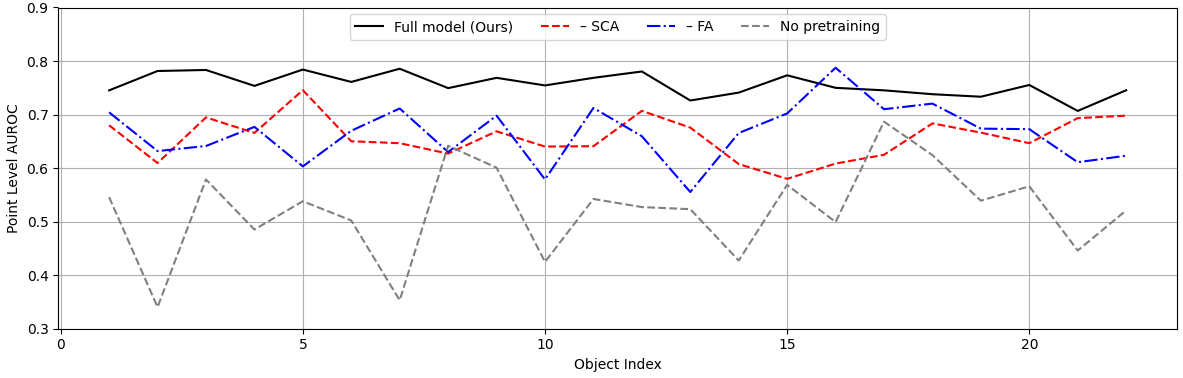
\includegraphics[width=0.9\linewidth]{figs/line1}
    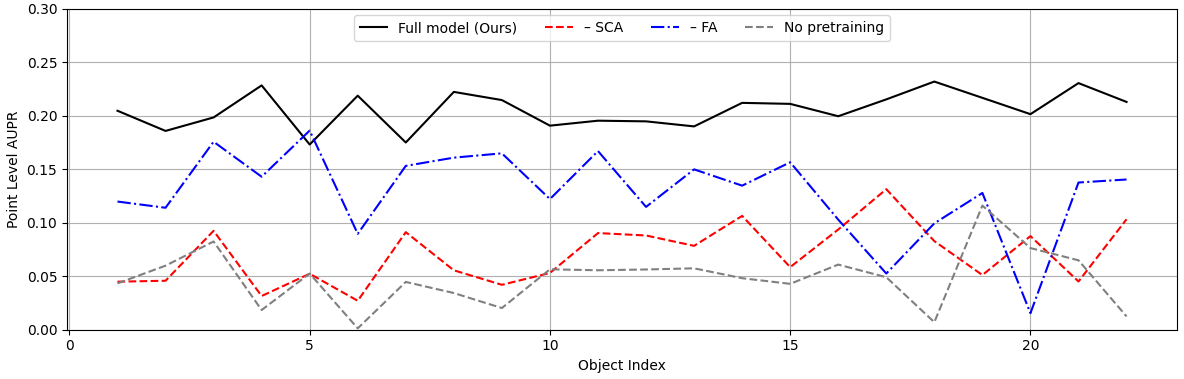
\includegraphics[width=0.9\linewidth]{figs/line2}
    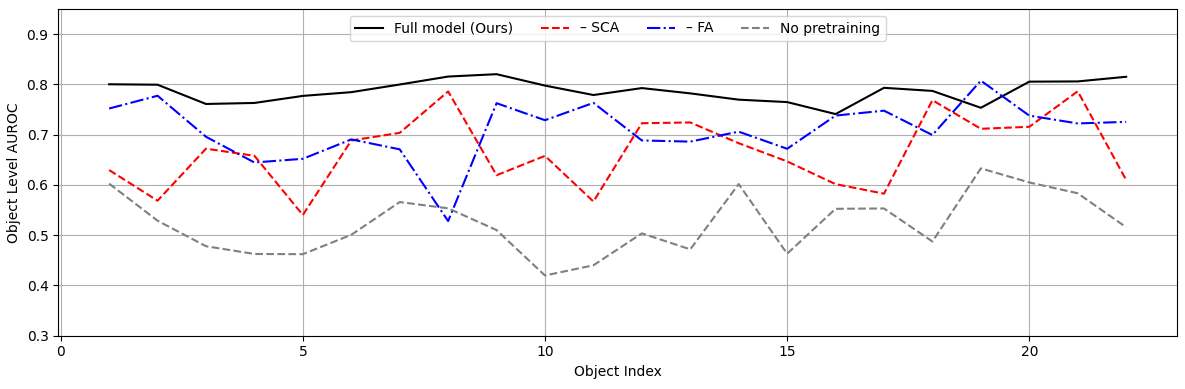
\includegraphics[width=0.9\linewidth]{figs/line3}
    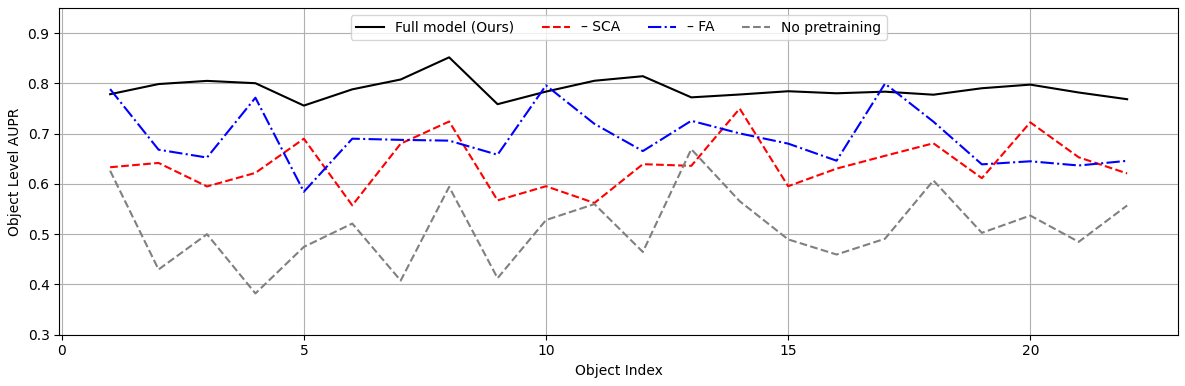
\includegraphics[width=0.9\linewidth]{figs/line4}
  \caption{Object- and point-level performance comparison across 22 test objects. Four line plots show (top left) point-level AUROC, (top right) point-level AUPR, (bottom left) object-level AUROC, and (bottom right) object-level AUPR for the full model (black solid) and three ablated variants (- SCA in red dashed; - FA in blue dash-dot; no pretraining in gray dashed).}
  \label{fig:ablation}
\end{figure}
%------------------------------------------------------------------

\begin{table}[ht]
\centering
\caption{Ablation Study: Average Results Across Datasets (AFG always present).}
\label{tab:Ablation}
\begin{tabular}{l|cc|cc|c}
\hline
& \multicolumn{2}{c|}{Point Level} & \multicolumn{2}{c|}{Object Level} & Speed \\
\hline
& AUROC & AUPR & AUROC & AUPR & FPS \\
\hline
Full model (Ours)          & 0.750 & 0.181 & 0.770 & 0.775 & 13.52 \\
- SCA                      & 0.719 & 0.103 & 0.715 & 0.707 & 18.66 \\
- FA                       & 0.735 & 0.169 & 0.752 & 0.756 & 14.79 \\
AFG (SimpleNet)            & 0.722 & 0.143 & 0.731 & 0.734 & 13.52 \\
Discriminator (SimpleNet)  & 0.724 & 0.132 & 0.725 & 0.729 & 14.15 \\
No global propagation      & 0.725 & 0.143 & 0.733 & 0.734 & 16.52 \\
No prototype snapping      & 0.743 & 0.165 & 0.755 & 0.760 & 14.22 \\
Pure geometry (no $W^z$)   & 0.731 & 0.149 & 0.734 & 0.736 & 14.46 \\
Pure feature (no $W^g$)    & 0.733 & 0.145 & 0.736 & 0.732 & 14.72 \\
No pretraining             & 0.504 & 0.053 & 0.525 & 0.530 & 13.52 \\
\hline
\end{tabular}
\end{table}

To quantify the impact of every design choice and hyperparameter in our pipeline, we conduct all ablations under the same training setups and baseline settings (frozen Point-MAE backbone; Spatial Context Aggregation with $\bar{n}=0.1n$, $K=10$, $\tau=0.5$, $\tau_c=0.1$; Feature Adaptor MLP hidden size $C/2$, residual weight $\alpha=0.5$; Anomalous Feature Generator corruption probability $p=0.5$ and noise standard deviation $\sigma=0.1$; 3D median filter radius 3 voxels at inference). We evaluate: (i) module removals: -- SCA (omit Spatial Context Aggregation) and -- FA (bypass the Feature Adaptor); (ii) SCA internals: No global propagation (skip inter-prototype fusion), No prototype snapping (disable final cosine re-assignment), Pure geometry (fuse only $W^g$) and Pure feature (fuse only $W^z$); (iii) learning setup: No pretraining (train transformer end-to-end); and (iv) core module baselines: AFG (SimpleNet), which perturbs all tokens with Gaussian noise rather than selectively, and Discriminator (SimpleNet), which replaces the attention-based discriminator with a per-token two-layer MLP.

Figure~\ref{fig:ablation} illustrates that our full model consistently delivers the best and most stable point- and object-level AUROC/AUPR across all 22 test objects. Table~\ref{tab:Ablation} reports the impact of each variant on average point- and object-level AUROC/AUPR as well as inference speed.

The full model achieves the highest performance across all metrics, attaining a point-level AUROC of 0.750 and AUPR of 0.181, along with object-level scores of 0.770 AUROC and 0.775 AUPR, while operating at 13.52 frames per second (FPS). Among all variants, removing the Spatial Context Aggregation (SCA) module leads to the most substantial performance degradation. Specifically, point-level AUROC and AUPR drop to 0.719 and 0.103, respectively, and object-level AUROC and AUPR fall to 0.715 and 0.707. Although inference speed improves to 18.66 FPS without SCA, the significant accuracy loss underscores the essential role of local-global fusion in enhancing the expressiveness of geometric features and capturing subtle surface anomalies.

Eliminating the Feature Adaptor (FA) results in a more moderate decline in detection quality. In this configuration, point-level AUROC and AUPR decrease to 0.735 and 0.169, while object-level AUROC and AUPR reduce to 0.752 and 0.756. The slight improvement in inference speed to 14.79 FPS suggests that the adaptor introduces only a marginal computational cost. Nevertheless, these results indicate that aligning the pretrained backbone features with the target industrial domain enhances anomaly separability and provides measurable gains in precision, even if it is not strictly indispensable.

We also compare our selective Anomalous Feature Generator with a variant inspired by SimpleNet, which perturbs all patch tokens uniformly by adding Gaussian noise. This modification leads to a clear performance drop: point-level AUPR declines from 0.181 to 0.143 and object-level AUPR from 0.775 to 0.734. These results validate the advantage of our selective corruption strategy, where only a random subset of tokens is perturbed. By introducing sparse and localized feature distortions, the generator produces harder negative samples that more accurately simulate realistic defects and improve the training signal for the discriminator.

Replacing our attention-based Discriminator with a SimpleNet-style per-token two-layer MLP leads to further degradation in performance. The point-level AUPR drops to 0.132 and object-level AUPR to 0.729, with a modest increase in speed to 15.85 FPS. This decline highlights the importance of joint reasoning across patch tokens: cross-patch attention enables the model to capture spatial dependencies and contextual relationships between patches, which are particularly important for identifying semantic inconsistencies and subtle geometric anomalies. In contrast, treating each token independently limits the model's ability to distinguish structural outliers that manifest only in relation to their neighbors.

Further ablations explore the internal mechanisms of the Spatial Context Aggregation module. Disabling global propagation between prototypes results in notable performance loss, with AUPR reduced to 0.143 at the point level and 0.734 at the object level, even though speed increases to 16.52 FPS. This confirms that long-range context transfer among prototypes contributes meaningfully to the model's ability to reason about distant but structurally related regions. Disabling the final prototype snapping or restricting fusion to only geometric ($W^g$) or only learned feature ($W^z$) affinities yields milder declines in detection quality. For all these variants, point-level AUROC remains above 0.731 and AUPR above 0.145, while object-level scores also stay above 0.732. These findings indicate that both affinity modalities are beneficial and that the soft re-assignment step, though not critical alone, adds refinement that enhances overall robustness.

Finally, removing the pretraining on ShapeNet and training the Point-MAE backbone from scratch results in a complete collapse in detection performance. The point-level AUROC and AUPR drop to 0.504 and 0.053, while object-level scores fall to 0.525 and 0.530, with no change in runtime. This stark contrast underscores the critical role of large-scale self-supervised pretraining in capturing generic 3D structural priors. Without this initialization, the model struggles to learn a meaningful notion of normalcy, especially under the weak supervision available in unsupervised anomaly detection.

This ablation study provides strong empirical support for our architectural choices. The Spatial Context Aggregation module and pretrained backbone are essential for accurate and reliable anomaly detection. The Feature Adaptor and global prototype interactions offer measurable improvements at minimal computational cost. Most notably, our selective pseudo-anomaly generation and attention-based discrimination outperform the corresponding SimpleNet variants by a clear margin, validating the core innovations of our method in terms of both accuracy and robustness in industrial 3D anomaly detection scenarios.

\section{Conclusion}

We have introduced an efficient framework for unsupervised 3D anomaly detection tailored for industrial applications. Our method combines a parameter-free Spatial Context Aggregation module, a lightweight Feature Adaptor for domain adaptation, and an Anomalous Feature Generator that synthesizes hard negatives in feature space. Built upon a pretrained Masked Autoencoder, the proposed approach effectively balances accuracy and efficiency without relying on memory banks or multi-pass inference. Our method achieves state-of-the-art results on both the Real3D-AD and Industrial3D-AD benchmarks. On Real3D-AD, we report a point-level AUROC of 0.763 and AUPR of 0.194, along with an object-level AUROC of 0.781 and AUPR of 0.775. On Industrial3D-AD, our framework achieves 0.730 AUROC and 0.184 AUPR at the point level, and 0.744 AUROC and 0.741 AUPR at the object level. These results reflect consistent improvements over the strongest prior baselines, with gains of up to 5.7\% in AUPR and 3.0\% in AUROC. Our pipeline also runs at 13.52 FPS, which, while not strictly real-time, represents a substantial speedup compared to existing 3D methods and is suitable for near-real-time inspection in industrial environments. In future work, we will optimize the model architecture and quantization schemes for deployment on edge devices to improve throughput in high speed production scenarios. We will also evaluate our approach with a wider variety of 3D sensors, such as structured light and time of flight cameras, to assess robustness under different noise and resolution characteristics. Finally, we plan to integrate our anomaly detector into robotic inspection systems and combine it with downstream tasks including 3D semantic mapping and automated manipulation to enable end to end quality control and corrective action in smart manufacturing environments.
